\chapter{Strategy}
\begin{figure}[H]
    \begin{tabular}{|l|p{12cm}|}
        \hline
        \textbf{Purpose} & \begin{itemize}
            \item To prioritize and order the analysis and design activities.
        \end{itemize} \\\hline
        \textbf{Concepts} & \begin{itemize}
            \item Requirements: A system's externally observable behavior.
            \item Conditions: The technical, organizational, and human oppirtunities and limites involved in performing a task.
        \end{itemize} \\\hline
        \textbf{Principles} & \begin{itemize}
            \item Tailor the strategy.
            \item Identify the difficult requirements and conditions.
            \item Maintain degrees of freedom.
        \end{itemize} \\\hline
        \textbf{Result} & \begin{itemize}
            \item A strategy for the analysis and design task.
        \end{itemize} \\\hline
    \end{tabular}
\end{figure}

\section{Characterize the Task}
\begin{description}
    \item[\textit{Problem domain}] Are you familiar with the type of target system? 
    \item[\textit{Application domain}] Are you familiar with the user organization?  
    \item[\textit{Technical platform}] Are you familiar with the technology?  
    \item[\textit{Development project}] How qualified are the developers? How good are the development conditions?  
    \item[\textit{Special conditions}] Which special conditions apply to this task?  
\end{description}

\begin{figure}[H]
    \centering
    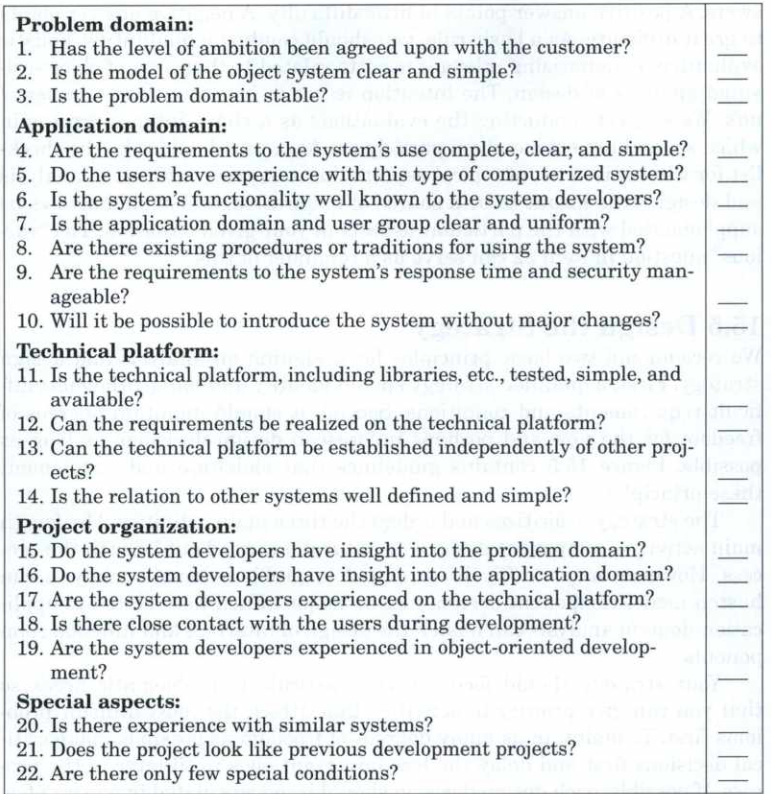
\includegraphics[width=\linewidth]{parts/6_practice/1_strategy/figures/checklist.png}
\end{figure}